\section{Unidad 2}

\subsection{Derivadas parciales}

La \textbf{derivada en un punto} \(P = (a,b)\),
de una función de una variable \(f(x)\),
devuelve la \textit{pendiente} \(m\),
de una recta que es tangente a \(f\) en el punto \(P\).

\vspace{.25cm}
\begin{equation*}
    \frac{df}{dx} = \lim_{\Delta x \to 0}\frac{\Delta y}{\Delta x} =
    \lim_{x \to a}\frac{f(x) - f(a)}{x-a}
\end{equation*}
\vspace{.25cm}

La derivada en funciones de dos variables sigue la misma idea:
aplicamos la derivada a cada una de las variables por separado,
considerando a la otra como constante.
Por eso hablamos de \textbf{derivada parcial}.

\begin{align*}
    \frac{\partial f}{\partial x} = f_x \\
    \\
    \frac{\partial f}{\partial y} = f_y \\
\end{align*}

Geométricamente,
podemos interpretar la derivada parcial respecto de \(x\)
en el punto \(P = (a, b, f(a,b))\),
como la \textit{pendiente} \(m\) de una recta tangente a la curva formada por
la intersección de \(f\) y el plano \(x = a\).
Lo mismo sucedería con la derivada parcial con respecto a \(y\).

\begin{figure}[H]
    \centering
    \caption{Interpretación geométrica de la derivada parcial}
    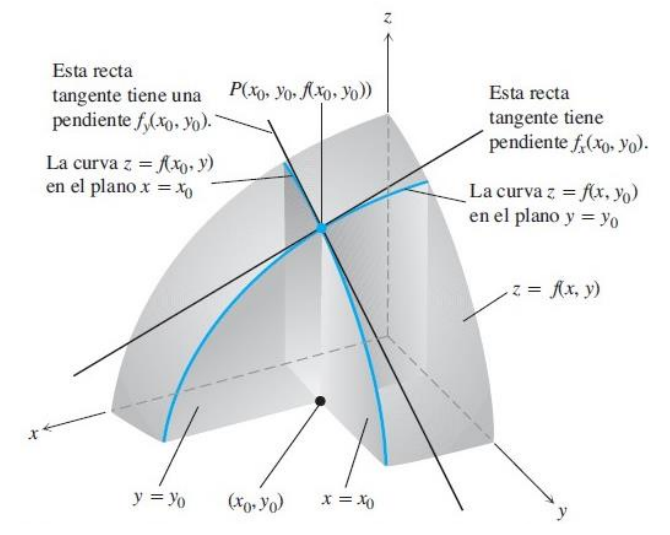
\includegraphics[scale=.8]{./img/01-02-derivada-parcial-geometrica.png}
\end{figure}

\vspace{.5cm}
\textbf{Ejemplo.}

Encontramos derivadas parciales de \(f(x,y) = x^{3} + x^{2}y^{3} - 2y^{2}\):

\begin{align*}
    f_x = 3x^{2} + 2xy^{3} \\
    f_y = 3x^{2}y^{2} - 4y \\
\end{align*}

\subsection{Propiedades y reglas de la derivada parcial}

\begin{enumerate}
    \item Con \(a\) constante:
          \begin{equation*}
              (a \cdot f)_x = a\cdot f_x
          \end{equation*}
    \item Distributiva respecto de la suma y resta:
          \begin{equation*}
              (f \pm g)_x = f_x \pm g_x
          \end{equation*}
    \item Regla del producto:
          \begin{equation*}
              (f\cdot g)_x = f_x\cdot g + f\cdot g_x
          \end{equation*}
    \item Regla del cociente:
          \begin{equation*}
              \left(\frac{f}{g}\right)_x = \frac{f_x\cdot g - f\cdot g_x}{g^{2}}
          \end{equation*}
    \item Regla de la cadena:
          Derivada parcial de \(g\), con \(f\) como está,
          por derivada parcial de \(f\):
          \begin{equation*}
              (g(f))_x = g(f)_x \cdot f_x
          \end{equation*}
\end{enumerate}

\subsection{Cálculo de derivada parcial por definición}

\subsubsection{Cuando la derivada no es continua en un punto}

Calculamos por definición,
manteniendo una constante.

\vspace{.5cm}
\textbf{Ejemplo.}

Calcular derivadas parciales de \(\sqrt[3]{x^{3} + y^{3}}\) en el origen:

Si calculamos derivada directamente:
\begin{align*}
    f_x & = \frac{1}{3}(x^{3} + y^{3})^{-2/3} \cdot 3x^{2} \\
    f_x & = \frac{x^{2}}{\sqrt[3]{(x^{3} + y^{3})^{2}}} \\
\end{align*}

Si evaluaramos esta derivada parcial en el origen,
encontraríamos una indeterminación.
Sin embargo, 
si derivamos por definición en el punto:

\begin{align*}
    f_x & = \lim_{x \to 0}\frac{f(x,0) - f(0,0)}{x - 0} \\
    f_x & = \lim_{x \to 0} \frac{\sqrt[3]{x^{3}} - 0}{x} \\
    f_x & = \boxed{1} \\
\end{align*}

Vamos con \(f_y\):

\begin{align*}
    f_y & = \lim_{y \to 0}\frac{f(0,y) - f(0,0)}{y - 0} \\
    f_y & = \lim_{y \to 0}\frac{y - 0}{y - 0} \\
    f_y & = \boxed{1}
\end{align*}

Aproximándonos por los ejes \(x\) e \(y\) la derivada tiende a \((1,1)\).


\subsubsection{Cuando está definida por partes}

Donde se da el cambio de función la derivada debe evaluarse por definición.

\vspace{.5cm}
\textbf{Ejemplo.}

Calcular derivada de:
\begin{align*}
    \begin{cases}
        \frac{3xy}{x^{2} + y^{2}} & (x,y)\neq (0,0) \\
        0 & (x,y) = (0,0)
    \end{cases}
\end{align*}

Calculamos por definición donde se produce el cambio de función:

\begin{align*}
     f_x & = \lim_{x \to 0}\frac{f(x,0) - f(0,0)}{x - 0} \\
     f_x & = \lim_{x \to 0}\frac{0 - 0}{x - 0} = \boxed{0} \\
\end{align*}

\begin{align*}
     f_y & = \lim_{y \to 0}\frac{f(0,y) - f(0,0)}{y - 0} \\
     f_y & = \lim_{y \to 0}\frac{0 - 0}{y - 0} = \boxed{0} \\
\end{align*}

La derivada por definición en el punto es \((0,0)\).

\subsubsection{Cuando puede que una exista y la otra no}

\subsubsection{En funciones de varias variables: derivabilidad \(\nRightarrow\) continuidad}

\subsection{Derivadas sucesivas}

Derivadas de \(2^{\circ}\) orden en varias variables:

\((f_x)_x = f_{xx}\).

\subsection{Teorema de Schwarz}

Si existen en torno al punto \(P\) \(f_x\),
\(f_y\)
y \(f_{xy}\),
con \(f_{xy}\) continua en \(P\),
\textbf{existe} \(f_{yx}\) y \(f_{yx}|_P = f_{xy}|_P\).

En concreto,
las derivadas cruzadas son iguales si la función es continua.

\subsection{Matrices especiales}

\subsubsection{Matriz jacobiana}

Matriz de las derivadas parciales de una o más funciones.

\subsubsection{Matriz Hessiana}

Matriz de las derivadas parciales \textit{de 2do orden}
de \textit{una} función.
Una función tiene \(2^{n}\) derivadas cruzadas si tiene 2 variables.

\subsection{Regla de la cadena}

Si \(f(x,y) = z\),
y podemos expresar x e y en función de t,
es decir, \(x(t), y(t)\),
se puede hacer una composición \(z(t)\).

Se puede componer y derivar \(\frac{dz}{dt}\) o, por regla de la cadena:

\begin{equation*}
    \frac{dz}{dt} = \frac{\partial z}{\partial x}\cdot\frac{dx}{dt} + \frac{\partial z}{\partial y}\cdot\frac{dy}{dt}
\end{equation*}

\subsection{Derivada direccional}

